Специфика эксперимента такова, что при заданном сдвиге по звёздной величине (или, что тоже самое, при заданном отношении усилений изображений) неопределённость во временной задержке, вызванная микролинзированием, не зависит от $\Delta t_{\textrm{ист.}}$. В действительности, в реально наблюдаемых изображениях гравитационно линзированных объектов нельзя точно указать отношение усилений, что нельзя не учитывать при более точных исследованиях. Для иллюстрации выбраны следующие значения: $$\Delta t_{\textrm{ист.}}=40, \ \Delta m = -0.28.$$
Для контроля точности временных интервалов между точками вводится сетка с $n=100$ делениями, так что частота отсчёта (расстояние вдоль горизонтальной оси между точками) составляет $\frac{400}{n}=4$ дня. (ТУТ). Модельная кривая блеска линейно интерполируется по этим точкам.
Сперва рассмотрим идеализированный случай, в котором кривая блеска в обоих изображениях "снимается", начиная с момента расширения сверхновой (Рис. \ref{fig:proba}a). В таком случае дисперсия очень маленькая: $\sigma_{\Delta t}=0.24$ дня. Это значение можно трактовать как нижнюю границу точности измерения временных задержек. Столь высокая точность объясняется следующими факторами: 

\begin{itemize}
    \item Высокая точность отсчёта,
    \item Постоянство погрешности измерения в формуле \eqref{chi2},
    \item Наличие характерной почти вертикальной части графика, обусловленной быстрым увеличением яркости сверхновой в первые дни после её взрыва.
\end{itemize}

Пусть теперь вертикальная часть охватывает меньший диапазон изменения блеска. В этом случае дисперсия резко возрастает и по порядку величины составляет несколько дней. ($\sigma_{\Delta t}=5.1$ дней, Рис. \ref{fig:proba}б). Если же ещё сильнее сдвинуть момент начала снятия кривой блеска, то дисперсия достигнет весьма больших значений ($\sigma_{\Delta t}=14.7$ дней, Рис. \ref{fig:proba}в, $\Delta t_{\textrm{ист.}}=60$).

Теперь смоделируем ситуацию, когда сверхновая детектируется после достижения пика своего блеска. Для реальных наблюдений сверхновых это наиболее реалистичная ситуация. В этом случае стандартное отклонение снова составляет несколько дней по порядку величины ($\sigma_{\Delta t}=2.7$ дней, Рис. \ref{fig:proba}г). 

Несмотря на широкий разброс в значениях, данные согласуются с работой \cite{doblerkeeton2006} -- в ней также показано, что временная задержка для измерений, в которых сверхновая детектируется после пика своей кривой блеска, имеет меньшую дисперсию, чем временная задержка для кривой блеска с характерным пиком. (ПОЧЕМУ)

(для первых трёх гистограмм) Такой рост в дисперсии $\Delta t$ объясняется тем, что флуктуации от микролинзирования наиболее сильно проявляются тогда, когда они совпадают по порядку величины с характерными изменениями истинной кривой блеска. 

\begin{figure}[H]
    \centering
	\begin{minipage}[h]{1.0\linewidth}
    \centering    
    	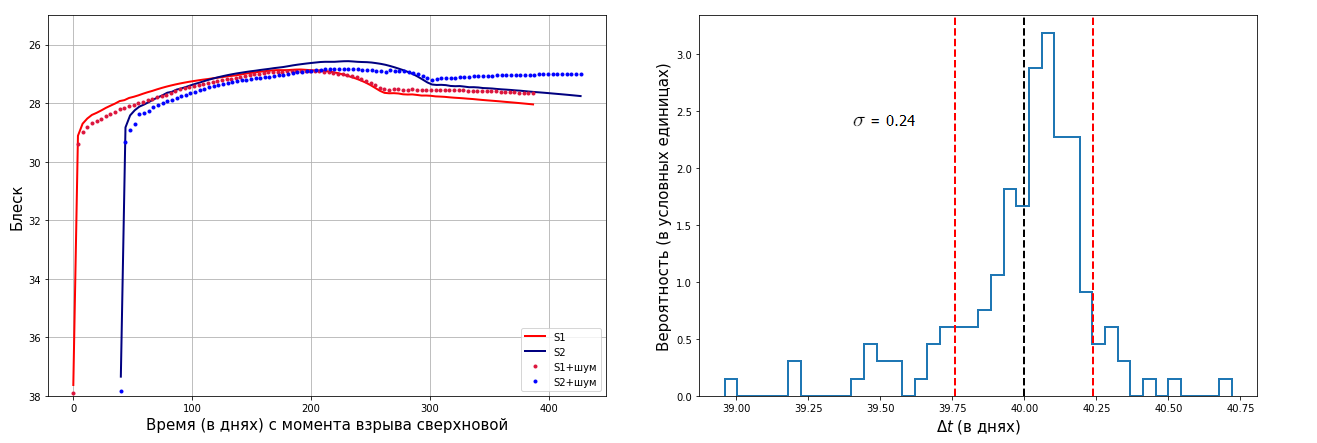
\includegraphics[scale=0.40]{pics/fig1.png} \\ \centering (а)  \\ 
	\end{minipage}
	\vfill
	\begin{minipage}[h]{1.0\linewidth}
	\centering
    	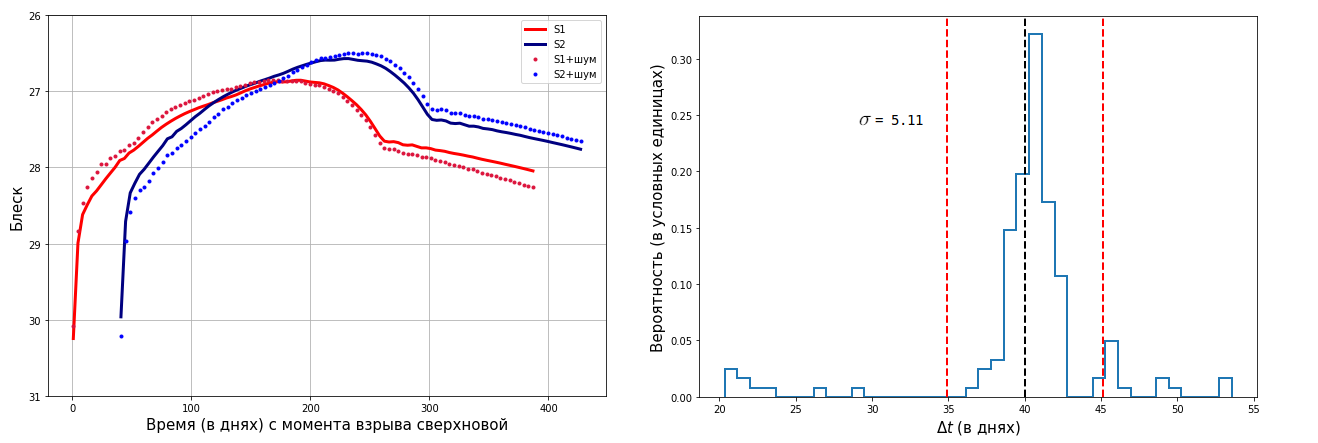
\includegraphics[scale=0.40]{pics/fig2.png} \\ \centering (б) \\
	\end{minipage}
	\vfill
	\begin{minipage}[h]{1.0\linewidth}
    \centering	
    	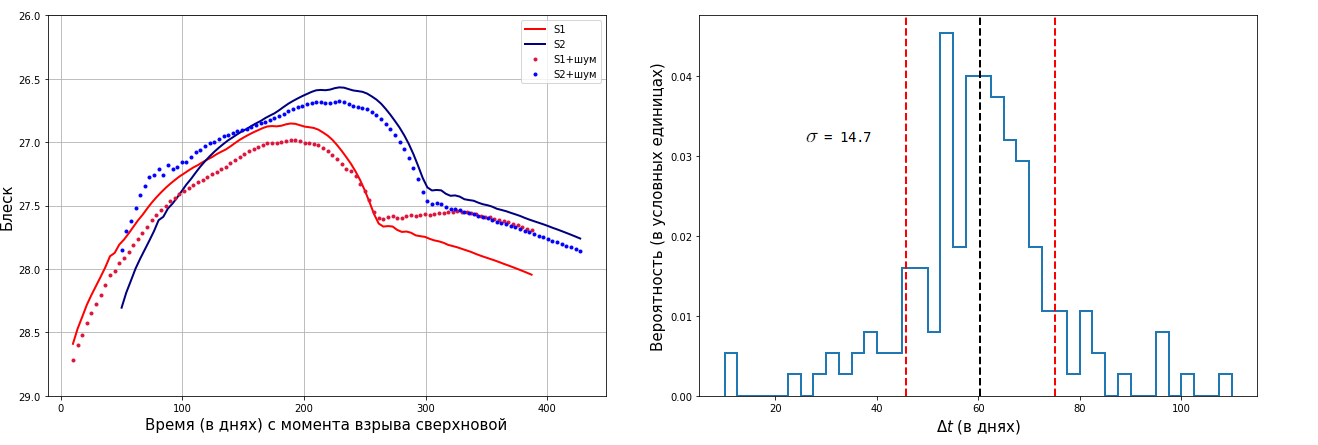
\includegraphics[scale=0.40]{pics/fig3.png} \\ \centering (в) \\
	\end{minipage}
	\vfill
	\begin{minipage}[h]{1.0\linewidth}
    \centering	
    	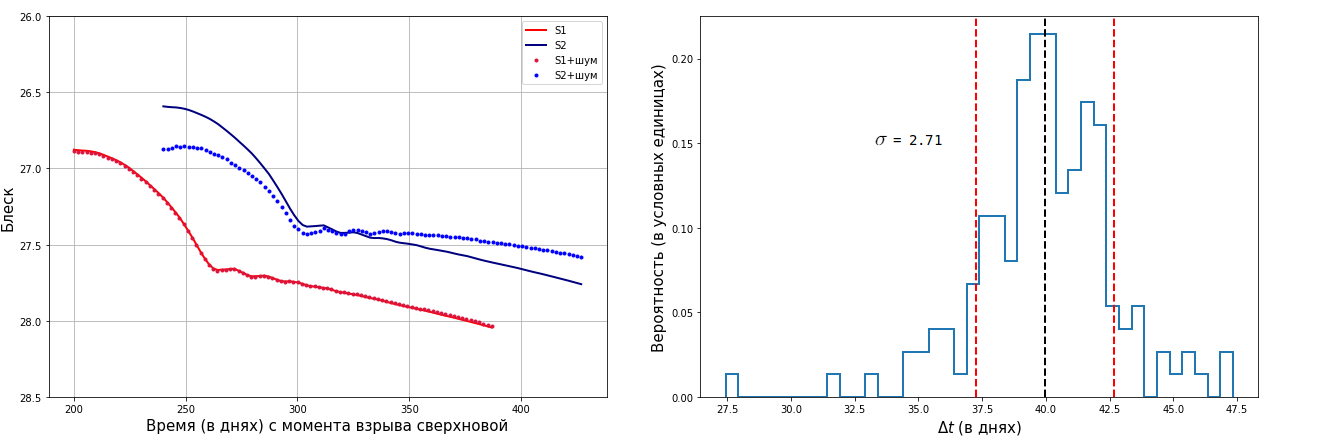
\includegraphics[scale=0.40]{pics/fig4.png} \\ \centering (г) \\
	\end{minipage}
	
	\caption{\textit{Слева}: кривые блеска в изображениях S1 и S2 SN Refsdal. Сплошной линией обозначены невозмущенные кривые блеска, точками -- одна из реализаций кривых блеска с шумами от микролинзирования. \textit{Справа}: гистограммы временных задержек для 150 измерений $\Delta t$. Чёрной пунктирной линией обозначено среднее по всем измерениям, красными пунктирными линиями - среднее плюс-минус одно стандартное отклонение. \label{fig:proba}} 
\end{figure}